\chapter{Implementierung}

Das Projekt ist in der Programmiersprache CSharp geschrieben.
Lokale Instanzen von Apache Kafka und Cassandra werden in Docker-Containern gestartet.
%TODO: Implementierung-Überblick


\section{Datenbankstruktur}

\begin{figure}[h!]%
    \centering%
    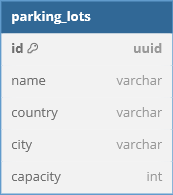
\includegraphics[width=0.3\textwidth]{Graphics/ParkingLotTable.png}%
    \caption{Parkhaus-Tabelle}%
    \label{fig:table_parking_lots}
\end{figure}%

In der Tabelle \ref{fig:table_parking_lots} sind alle Parkhäuser, die im System existieren mit ihrem Standort, sowie ihrer Kapazität, hinterlegt.
Die Daten hierin werden aktuell manuell angelegt.

\begin{figure}[h!]%
    \centering%
    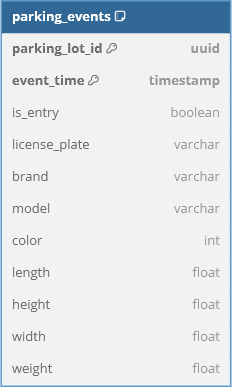
\includegraphics[width=0.3\textwidth]{Graphics/parking_events.png}%
    \caption{Parkevent-Tabelle}%
    \label{fig:table_parking_events}
\end{figure}%

In der Tabelle \ref{fig:table_parking_events} sind alle in der Vergangenheit geschehenen Park-Events gespeichert.
Bei diesen Daten handelt es sich um reine Rohdaten, die den unverarbeiteten Daten von Parkhäusern entsprechen.

\begin{figure}[h!]%
    \centering%
    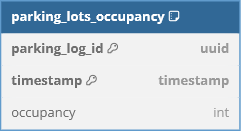
\includegraphics[width=0.3\textwidth]{Graphics/occupancy.png}%
    \caption{Zwischensummen-Tabelle}%
    \label{fig:table_occupancy}
\end{figure}%

In der Tabelle \ref{fig:table_occupancy} werden Füllstände der Parkhauser zu bestimmten Zeitpunkten gespeichert.
Diese Daten werden periodisch vom Batch-Layer inkrementell berechnet und können bei Bedarf, beispielsweise nach Rohdaten-Korrektur oder Batch-Prozess-Korrektur nochmal über alle Daten hinweg neu berechnet werden.

\section{Core-Bibliothek}
Auf der Core-Bibliothek bauen alle anderen Projekte auf.
In dieser Bibliothek befinden sich alle geteilten Programmteile:
\begin{itemize}
    \item \textbf{Konfiguration}: string Konstanten für Kafka-Topics, sowie Cassandra-Aufbau bestehend aus Tabellen und -Spaltennamen
    \item \textbf{Geteilte Interfaces}: ICarModel (allgemeine Autoinformationen), ICarData (ICarModel + spezifische Autoinformationen), IParkingEventData (ICarData + Parkhaus + Einfahrts- oder Ausfahrtszeit)
    \item \textbf{Geteilte Datenstrukturen}: CarEntryData (rerpäsentiert ein vollständiges Einfahrts-Event), CarExitData (rerpäsentiert ein vollständiges Ausfahrts-Event), OccupancyState (repräsentiert den exakten Füllstand eines Parkhauses zu einem gegebenen Zeitpunkt)
    \item \textbf{Serialisierungs- und Deserialisierungsfuntionen}: Datenstrukturen binär oder als String serialisieren und wiedererstellen
    \item \textbf{CassandraHelper}: Hilfsklasse, die die Verbindung zur Cassandra-Datenbank verwaltet und alle in anderen Projekten verwendeten Datenbankzugriffe mit Hilfe von CQL (Cassandra Query Language) umsetzt
    \item \textbf{Setup-Validierung}: ermöglicht Anwendungen, die Kafka oder Cassandra benötigen zu überprüfen, ob Kafka und Cassandra korrekt aufgesetzt sind, bevor sie starten
\end{itemize}


\section{Datengrundlage}
Da keine realen Daten zur Verfügung stehen, verwenden wir einen selbst geschriebenen Datengenerator, der Ein- und Ausfahrten in ein Parkhaus über Zeit simuliert.
Dabei werden Parkevent-Daten \quotes{CarEntryData} und \quotes{CarExitData} bestehend aus Parkhaus-Id, Zeitstempel, Nummernschild, Automarke, Automodell, Farbe, gemessener Länge, gemessener Breite, gemessener Höhe und gemessenem Gewicht generiert.
Die Parkevent-Daten werden dann direkt in die Kafka-Topic \quotes{car-events} geschrieben.
Ausfahrts-Events werden stets basierend auf einem zuvor generierten Einfahrts-Event, zu dem es noch kein zugehöriges Ausfahrts-Event gibt generiert.
Dieser Prozess geschieht stark beschleunigt, um einfaches Testen zu ermöglichen: Innerhalb von Minuten werden Daten für einen ganzen Tag generiert.
Um die Daten für mehrere Parkhäuser auf einmal zu generieren, können beliebig viele Parkhäuser konfiguriert werden.
Für jedes Parkhaus wird dann ein entsprechender Generator-Thread gestartet.
Der Generator berücksichtigt die maximale Kapazität eines Parkhaus und generiert morgens mehr Einfahrts-Events und abends mehr Ausfahrts-Events.
%Todo: Tabelle angeben
In der Datenbank stehen Einfahrts- und Ausfahrts-Events in der selben Tabelle und werden nur durch ein bool-Flag, bei dem \textbf{True} ein Einfahrts-Event markiert, unterschieden.


\section{Speed Layer}
Der Speed Layer beinhaltet nur ein einzelnes Projekt \quotes{SpeedLayerParkingDeckWorker}, das gleichzeitig Kafka-Consumer und Kafka-Producer ist.
Dabei handelt es sich um eine Kommandozeilenanwendung, die die eingehenden Grunddaten aus der Kafka-Topic \quotes{car-events} erhält und für ein einzelnes Parkhaus mehrere Events zu einer Zwischensumme zusammenfasst.
Diese Zwischensumme entspricht der Differenz der im Parkhaus stehenden Autos im Vergleich zum Stand vor den Events.
Wird eine Obergrenze an Park-Events für ein Parkhaus erreicht, oder ist eine Zeitspanne seit dem ersten Park-Event abgelaufen, so wird die Differenz gemeinsam mit der Parkhaus-Id in eine zweite Kafka-Topic \quotes{car-events-preprocessed} geschrieben.
Die Obergrenze an Parkevents, sowie die Zeitspanne sind im Worker konfigurierbar.
Es können beliebig viele Speed-Layer-Worker gleichzeitig gestartet werden, wobei je Parkhaus ein Speed-Layer-Worker vorgesehen ist.
Standardmäßig wird beim Starten des Projekts auch ein Worker je Parkhaus gestartet.
Durch die Verwendung der selben GruppenId (abhängig vom Parkhaus des Workers) ist es auch möglich, mehrere Worker für das selbe Parkhaus zu starten, während Kafka jedes Event nur an einen dieser Worker verteilt.
Praktisch ist das in unserer Fallstudie allerdings nicht sinnvoll, da ein einzelnes reales Parkhaus nur eine überschaubare Menge an Events produzieren kann.


\section{Batch Layer}
%TODO: Projektnamen in Repo anpassen
Das Batch Layer besteht aus mehreren Projekten:
\begin{itemize}
    \item \textbf{Kafka-Consumer} persistiert alle Grunddaten aus Kafka in der Datenbank.
    \item \textbf{Batch-Processing} führt regelmäßig verschiedene Batch-Berechnungen basierend auf den in der Datenbank persistierten Daten aus und schreibt die Ergebnisse in die Datenbank zurück. 
\end{itemize}

\subsection{KafkaConsumer}
Der Kafka-Consumer des Batch Layers ist eine Kommandozeilenanwendung, die beim Start die Kafka-Topic \quotes{car-events} abonniert und alle hier anfallenden Events erhält.
Diese Events werden dann in Cassandra übertragen, das geschieht der Einfachheit halber aktuell in einzelnen Datenbankoperationen.
In einem realen System, in dem mehr Daten anfallen, wäre hingegen wichtig, die Events zu bündeln und eine Menge Events gesammelt an die Datenbank zu übertragen.
Es können beliebig viele Kafka-Consumer gleichzeitig gestartet werden.
Alle Instanzen teilen die selbe Kafka-GroupId, wodurch jedes Event nur an genau eine Instanz übertragen wird.
In der Kommandozeile werden Ein- und Ausfahrten ausgegeben.

\subsection{Batch-Processing}
Das Batch-Processing des Batch Layers ist eine Kommandozeilenanwendung, die periodisch die Daten der vergangenen halben Stunde aus der Datenbank läd und darauf basierend Zwischenfüllstände je Parkhaus je 10 Minuten berechnet.
Da der Datengenerator beschleunigt Daten generiert, läuft diese Anwendung auch beschleunigt und berechnet alle 2 Minuten die Daten einer halben Stunde.



\section{Serving Layer}
Das Serving Layer besteht nur aus einem Projekt \quotes{ServingLayer}.
Hier handelt es sich um eine Kommandozeilenanwendung, die Daten aus Kafka und Cassandra zusammenführt und für Benutzeranwendungen bereitstellt.
Beim Start liest der Serving Layer alle existierenden Parkhäuser aus der Cassandra-Datenbank und legt sich je Parkhaus einen Cache an.
Dazu werden die Kafka-Topics \quotes{car-events-preprocessed}, deren Daten im Speed Layer berechnet werden, und \quotes{batch-notification} abonniert.
Dieser Cache beinhaltet die aktuelle Anzahl an Autos im Parkhaus, die sich aus dem Ergebnis der letzten Batch-Zwischensumme, sowie der seitdem angefallenen Summe an Park-Events in \quotes{car-events-preprocessed} ergibt.
Immer wenn eine Nachricht in \quotes{batch-notification} den Abschluss eines weiteren Batch-Vorgangs signalisiert, wird die aktuelle Batch-Zwischensumme neu geladen, sowie der veraltete Teil der Speed Layer Daten aus \quotes{car-events-preprocessed} verworfen.
Aufgrund des Aufbaus des Speed-Layers, sowie der asynchronen Natur von Batch- und Speed-Layer kann ein Ergebnis des Speed-Layers Daten aus 2 Batch-Berechnungen beinhalten.
Das kann zu temporären Inkonsistenzen führen, die aber nach der nächsten Batch-Berechnung korrigiert sind.
Anwendungen können die Daten vom Serving Layer über TCP/IP abfragen.
Wenn Historische Daten, die sich nicht im Cache befinden, wie Füllstände über Zeit abgefragt werden, leitet das Serving Layer die Anfrage an die Cassandra-Datenbank durch.

\section{Frontend}
Das Frontend ist in Avalonia 
%Avalonia
%nur mit 
